\chapter{RStudio: une introduction}
\label{rstudio}


\section{Installation}
\label{rstudio:installation}



\section{Description sommaire}
\label{rstudio:description}


\begin{figure}[t]
  %% Capture d'écran
  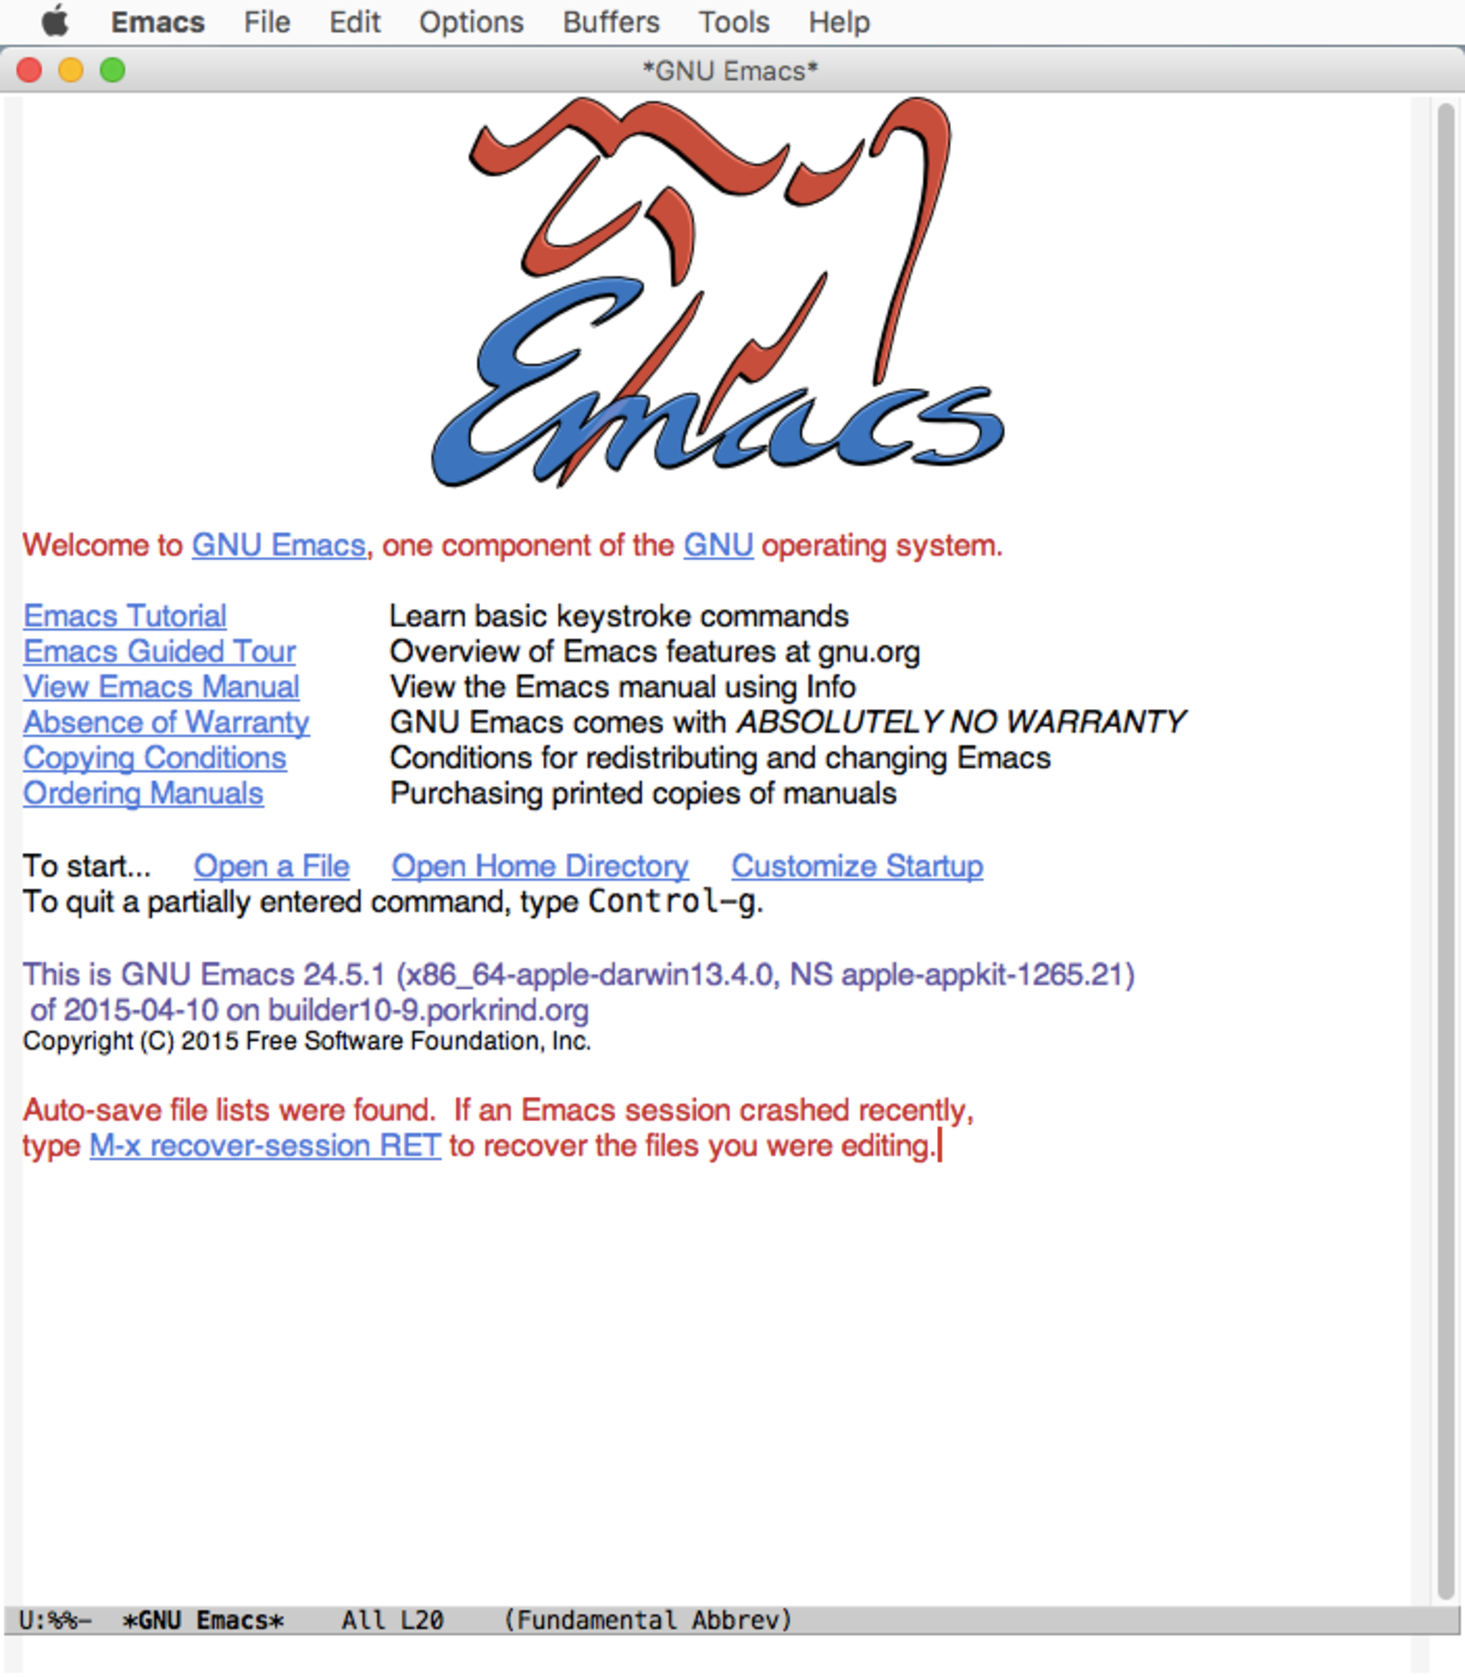
\includegraphics{emacswindow-screenshot}

  %% Identification du minibuffer
  \begin{textblock}{0.35}(7.35,-0.08)
    \LARGE$\leadsto$
  \end{textblock}
  \begin{textblock}{1.75}(7.85,-0.1)
    \small \emph{Minibuffer}
  \end{textblock}

  %% Identification de la barre de menu
  \begin{textblock}{0.35}(7.35,-6.58)
    \LARGE$\leadsto$
  \end{textblock}
  \begin{textblock}{1.75}(7.85,-6.6)
    \small Barre de menu
  \end{textblock}

  %% Identification du buffer
  \begin{textblock}{0.35}(7.35,-3.38)
    \LARGE$\leadsto$
  \end{textblock}
  \begin{textblock}{1.75}(7.85,-3.4)
    \small \emph{Buffer}
  \end{textblock}

  %% Identification de la mode line
  \begin{textblock}{0.35}(7.35,-0.28)
    \LARGE$\leadsto$
  \end{textblock}
  \begin{textblock}{1.75}(7.85,-0.3)
    \small Ligne de mode
  \end{textblock}
  \caption{Fenêtre GNU~Emacs et ses différentes parties au lancement
    de l'application sous Mac OS~X. Sous Windows et Linux, la barre de
    menu se trouve à l'intérieur de la fenêtre.}
  \label{fig:ess:emacswindow}
\end{figure}



\begin{figure}[t]
  \begin{osx}
    Par défaut sous Mac OS~X, la touche \code{Meta} est assignée à
    \code{Option} (\optkey). Sur les claviers français, cela empêche
    d'accéder à certains caractères spéciaux tels que [, ], \{ ou \}.

    Une solution consiste à plutôt assigner la touche \code{Meta} à
    \code{Commande} (\cmdkey). Cela bloque alors l'accès à certains
    raccourcis Mac, mais la situation est moins critique ainsi.

    Pour assigner la touche \code{Meta} à \code{Commande} (\cmdkey) et
    laisser la touche \code{Option} (\optkey) jouer son rôle usuel, il
    suffit d'insérer les lignes suivantes dans son fichier de
    configuration \code{.emacs} (voir la
    \autoref{emacs+ess:configuration}):
\begin{verbatim}
;;; ====================================
;;;  Assigner la touche Meta à Commande
;;;  et laisser Option être Option
;;; ====================================
(setq-default ns-command-modifier 'meta)
(setq-default ns-option-modifier 'none)
\end{verbatim}
  \end{osx}
  \label{fig:ess:meta}
\end{figure}



\section{Commandes de base}
\label{rstudio:commandes}



\section{Anatomie d'une session de travail (bis)}
\label{rstudio:session}

On reprend ici les étapes d'une \capsule{http://youtu.be/xiNnHegDau8}{session de
  travail} type présentées à la \autoref{presentation:session}, mais
en expliquant comment compléter chacune dans Emacs avec le mode ESS.

\begin{enumerate}
\item Lancer Emacs et ouvrir un fichier de script avec
  \begin{quote}
    \code{C-x C-f}
  \end{quote}
  ou avec le menu
  \begin{quote}
    \code{File|Open file...}
  \end{quote}
  En spécifiant un nom de fichier qui n'existe pas déjà, on se trouve
  à créer un nouveau fichier de script. S'assurer de terminer le nom
  du nouveau fichier par \code{.R} pour que Emacs reconnaisse
  automatiquement qu'il s'agit d'un fichier de script R.
\item Démarrer un processus R à l'intérieur même de Emacs avec
  \begin{quote}
    \code{M-x R }\returnkey
  \end{quote}
  Emacs demandera alors de spécifier de répertoire de travail
  (\emph{starting data directory}). Accepter la valeur par défaut, par
  exemple
  \begin{quote}
    \verb=~/ =\returnkey
  \end{quote}
  ou indiquer un autre dossier. Un éventuel message de Emacs à l'effet
  que le fichier \code{.Rhistory} n'a pas été trouvé est sans
  conséquence et peut être ignoré.
\item Composer le code. Lors de cette étape, on se déplacera souvent
  du fichier de script à la ligne de commande afin d'essayer diverses
  expressions. On exécutera également des parties seulement du code se
  trouvant dans le fichier de script. Les commandes les plus utilisées
  sont alors
  \begin{quote}
    \ess{C-RET}\ pour exécuter une ligne du fichier de script; \\
    \ess{C-c C-c}\ pour exécuter un paragraphe du fichier de script; \\
    \emacs{C-x o}\ pour se déplacer d'une fenêtre à l'autre; \\
    \ess{C-c C-e}\ pour replacer la ligne de commande au bas de la
    fenêtre.
  \end{quote}
\item Sauvegarder le fichier de script:
  \begin{quote}
    \emacs{C-x C-s}
  \end{quote}
  Les quatrième et cinquième caractères de la ligne de mode changent
  de \,\verb|**|\, à \,\verb|--|.
\item Sauvegarder si désiré l'espace de travail de R avec
  \code{save.image()}\indexfonction{save.image}. On le répète, cela
  n'est habituellement pas nécessaire à moins que l'espace de travail
  ne contienne des objets importants ou longs à recréer.
\item Quitter le processus R avec
  \begin{quote}
    \ess{C-c C-q}
  \end{quote}
  Cette commande ESS se chargera de fermer tous les fichiers associés
  au processus R. On peut ensuite quitter Emacs en fermant
  l'application de la manière usuelle.
\end{enumerate}



\section{Configuration de l'éditeur}
\label{rstudio:configuration}



\section{Aide et documentation}
\label{rstudio:aide}


%%% Local Variables:
%%% mode: latex
%%% TeX-master: "introduction_programmation_r"
%%% coding: utf-8
%%% End:
